\section{Wirkungsgradberechnung}
\label{cha:wgberechnung}
Betrachtet man den Kreisprozess der Gasturbine - den Joule-Prozess - findet in der Turbine eine isentrope Entspannung bzw. Expansion statt. Aus dem ersten Hauptsatz der Thermodynamik ergibt sich mit adiabater Zustandsänderung und unter Vernachlässigung der Reibungsverluste die von der Turbine an den Verdichter abgegebene Leistung zu
\begin{equation}
\label{eq:leistungTurbine}
P = \dot m (h_{t5} - h_{t4})
\end{equation}
wobei $h_{t5}$ die Totalenthalpie am Turbinenaustritt und $h_{t4}$ die Totalenthalpie am Turbineneintritt ist. 



%__________________________
\subsection{Wirkungsgrad allgemein}

Wie in Abb. \ref{fig:hsTurbine} zu sehen, ergibt sich der isentrope Wirkungsgrad aus dem Verhältnis der verlustbehafteten und der isentropen Enthalpiedifferenz bzw. dem Verhältnis der Turbinenleistungen zu:

\begin{equation}
\label{eq:leistungTurbine}
\overline{\eta}_{t} = \frac{h_{t5} - h_{t4}}{\overline{h}_{t5} - h_{t4}} =  \frac{P}{ \overline{P}} 
\end{equation}

\begin{figure}[htbp]
	\centering
	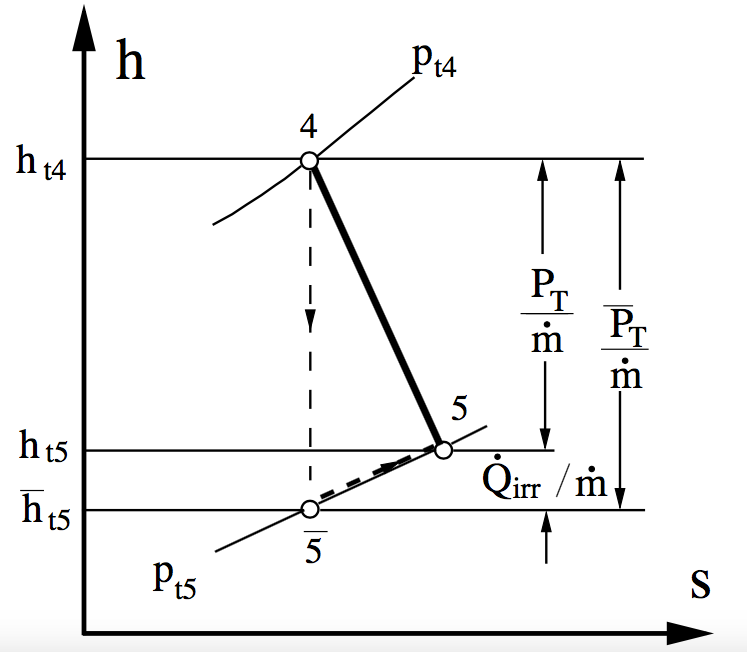
\includegraphics[width=0.5\textwidth]{hsTurbine.png}
	\caption{h-s-Diagramm der Turbine} \label{fig:hsTurbine}
	
\end{figure} 

Oder umformuliert mit der isentropen Totalenthalpiedifferenz dargestellt durch $\Delta H_{t_{is}} = \overline{h}_{t5} - h_{t4}$ zu:
\begin{equation}
\label{eq:wgallgemein}
\eta =\frac{P}{\Delta H_{t_{is}}}
\end{equation}

Die isentrope Enthalpiedifferenz $\Delta H_{t_{is}}$ wird nach
\begin{equation}
\label{eq:wgnenner}
\Delta H_{t_{is}} = \dot m \cdot c_p \cdot T_{t_{inlet}} \cdot \left[ \left( \frac{p_{t_{outlet}}}{p_{t_{inlet}}}\right)^\frac{\gamma-1}{\gamma}-1\right]
\end{equation}
mit dem Massenstrom $\dot m$, der spezifischen Wärmekapazität bei konstantem Druck $c_p$ (siehe Berechnungsweise Abschnitt \ref{subsec:spezWK}), der Totaltemperatur am Inlet $T_{t_{inlet}}$, dem Totaldruck am Inlet $p_{t_{inlet}}$, dem Totaldruck am Outlet $p_{t_{outlet}}$ und dem Isentropenexponenten $\gamma$ berechnet.\newline 
Im folgenden Abschnitt werden verschiedene Definitionsmöglichkeiten für die erzeugte Leistung $P$ vorgestellt.
%__________________________
\subsection{Erzeugte Leistung}
\label{sec:wirkungsgrade}
Die erzeugte Leistung $P$ im Zähler der Gleichung \ref{eq:wgallgemein} für den Wirkungsgrad  lässt sich unter anderem mit einer der drei folgenden Gleichungen berechnen:\newline
Mit Hilfe der tatsächlichen Totaltemperaturdifferenz $\Delta T_t$ und der spezifischen Wärmekapazität $c_p$ nach:
\begin{equation}
\label{eq:wgzaehlertt}
P_{\Delta T_t} = \dot m \cdot c_p \cdot \Delta T_t = \dot m \cdot c_p \cdot \left( T_{t_{inlet}}-T_{t_{outlet}} \right),
\end{equation}
mit Hilfe der Totalenthalpie am Inlet $h_{t_{inlet}}$ und Outlet $h_{t_{outlet}}$, welche direkt aus ANSYS CFX entnommen wird, nach:
\begin{equation}
\label{eq:wgzaehlerht}
P_{\Delta h_t} = \dot m \cdot \Delta h_t = \dot m \cdot \left( h_{t_{inlet}}-h_{t_{outlet}} \right)
\end{equation}
oder mit Hilfe des Momentes $M_{Rotor}$ um die Rotationsachse an Schaufel und Hub des Rotors, der Anzahl Rotoren $N_{Rotor}$ und der Winkelgeschwindigkeit des Rotors $\omega_{Rotor}$ nach:
\begin{equation}
\label{eq:wgzaehlertorque}
P_{torque} = M_{Rotor} \cdot N_{Rotor} \cdot \omega_{Rotor}
\end{equation}
Da auch die Berechnung der spezifischen Wärmekapazität $c_p$ aus den Gleichungen \ref{eq:wgnenner} und \ref{eq:wgzaehlertt} Einfluss auf den Wirkungsgrad haben kann, wird im kommenden Abschnitt näher auf dessen Definition eingegangen.

\subsubsection{Spezifische Wärmekapazität}
\label{subsec:spezWK}
Die spezifische Wärmekapazität bei konstantem Druck $c_p$ ist eine temperaturabhängige Größe. Wenn die Temperaturdifferenz zwischen In- und Outlet sehr groß ist, verändert sich $c_p$ zwischen In- und Outlet wesentlich und kann somit nicht mehr als konstant angenommen werden. Die temperaturabhängige Wärmekapazität $c_p$ lässt sich mit dem folgenden Polynom in Abhängigkeit der Temperatur $T$ berechnen, zu sehen in Abbilgung \ref{fig:cpPlot}.  
\begin{equation}
\label{eq:cppolynom}
c_p = \frac{a\cdot T^4-b\cdot T^3+c\cdot T^2-d\cdot T+e}{f}\frac{J} {kg \cdot K}
\end{equation}
Die Konstanten $a$ bis $f$ sind der folgenden Tabelle \ref{tab:cpparameter} zu entnehmen.
\begin{table}[H]
\centering
\caption{Konstanten für die Berechnung von $c_p$} \label{tab:cpparameter}
\begin{tabular}{ c| c|c|c|c|c}
$a$&$b$&$c$&$d$&$e$&$f$\\
\hline
$0.12934K^{-4}$&$596.633K^{-3}$&$933833K^{-2}$&$373,61\cdot10^6K^{-1}$&$105,01\cdot10^{10}$&$10^9$\\
\end{tabular}

\end{table}

\begin{figure}[htbp]
	\centering
	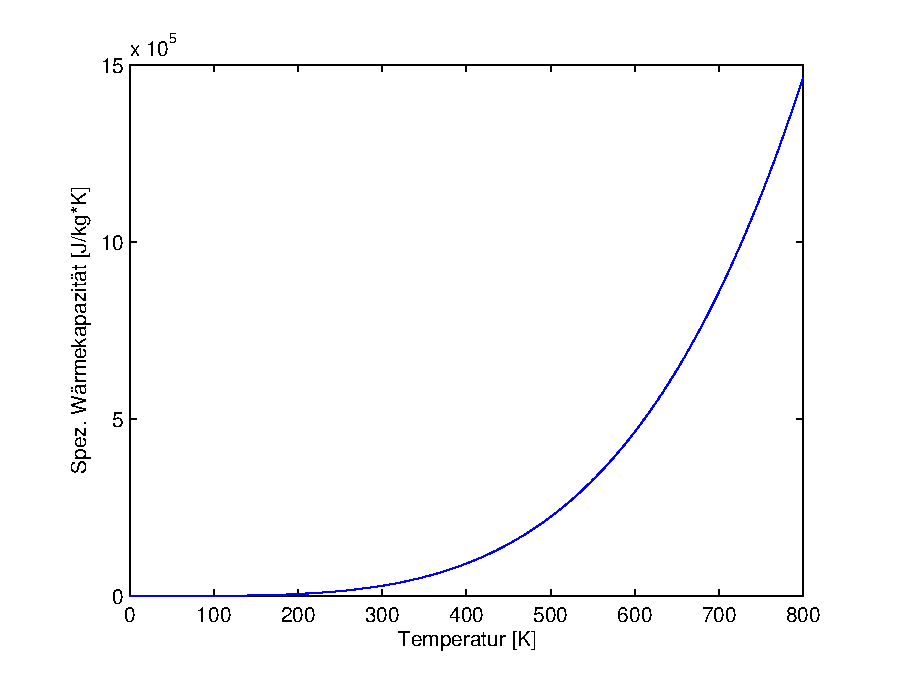
\includegraphics[width=0.8\textwidth]{cp_Plot.eps}
	\caption{Spez. Wärmekapazität temperaturabhängig} \label{fig:cpPlot}
	
\end{figure} 

Bei der Berechnung der isentropen Enthalpiedifferenz $\Delta H_{t_{is}}$ aus Gleichung \ref{eq:wgnenner} wurde $c_p$ nach Gleichung \ref{eq:cppolynom}
\begin{itemize}
	\item separat am In-/Outlet: $c_{p_1} = c_p(T_1)\, ;\, c_{p_3} = c_p(T_3)$,
	\item in Abhängigkeit der isentropen Temperatur im Outlet: $c_{p_3}^* = c_{p_3}(T_{3_{is}})$,
	\item aus dem arithmetischen Mittel der beiden Größen: $\bar{c_p} = \frac{c_{p_1} + c_{p_3}}{2}\, ;\, \bar{c_p^*} = \frac{c_{p_1} + c_{p_3}^*}{2}$
	
\end{itemize}
berechnet um den Einfluss der Berechnungsweise von $c_p$ auf die Berechnung des Wirkungsgrades zu analysieren.\\

Die verschiedenen Wirkungsgraddefinitionen in Abschnitt \ref{sec:wirkungsgrade} und Berechnungsweisen von $c_p$ wurden in CFX implementiert und miteinander verglichen. Das Ergebnis dieses Vergleichs wird im nächsten Abschnitt dargestellt.
%__________________________

\begin{comment}
\section{Wirkungsgrade bei der Aachen-Turbine}
\label{sec:wgaachen}
Bei der Aachen-Turbine ergaben sich je nach Berechnungsart folgende Werte für den Wirkungsgrad:
\begin{table}[H]
\centering
\caption{Wirkungsgrad bei der Aachen-Turbine}
\begin{tabular}{ c| c}
Berechnungsformel & $\eta$ \\
\hline
$\eta_{\Delta T_t}$ mit $c_p$ konstant& 86\% \\
$\eta_{\Delta T_t}$ mit $c_p(T)$& 86\% \\
$\eta_{\Delta h_t}$& 87\% \\
$\eta_{torque}$& 85\% \\
\end{tabular}
\label{tab:wgaachen}
\end{table}
Es ist zu sehen, dass .....
\todo
\end{comment}




%%% Local Variables: 
%%% mode: latex
%%% TeX-master: "main"
%%% End: 


